\documentclass[12pt]{article}
\usepackage[left=.5in, right=.5in, top=.5in, bottom=.5in]{geometry}
\usepackage[parfill]{parskip}
\usepackage{amsmath, amssymb, graphicx, svg}
\pagenumbering{gobble}
\setlength\parindent{0pt}
\newcommand{\m}[1]{\mathbf{#1}}
\newcommand{\mhat}[1]{\hat{\mathbf{#1}}}

\begin{document}

\begin{center}
{\Large CSC413H1 - Assignment 2}
\end{center}

\textbf{1.1.1:} Each $\mathcal{B}$ is randomly sampled without replacement from the rows of $X$, so it lies in the row space of $X$. Next, since $\nabla_{\m w_t} \mathcal{L}(\m x_j,\m w_t) = \nabla_{\m w_t} \frac{1}{n}||\m w_t^T \m x_j - \m t_j||^2_2 = \frac{2}{n}||\m w_t^T \m x_j - \m t_j||^2_2 \m x_j$ is a scalar multiple of $\m x_j$, every update is a linear combination of rows in $X$ and thus stays within the span of $X$. This implies that the mini-batch SGD solution $\mhat w$ is in the span of $X$, and similar to in Assignment 1 we can write $\mhat w = X^T\m a$ for some $\m a \in \mathbb{R}^n$. Then, for any other solution $\m w' \in \mathbb{R}^d$ where $X\m w' = \m t$, notice that \begin{align*}
    (\mhat w - \m w')^T\mhat w = (\mhat w - \m w')^T X^T\m a = (X\mhat w - X\m w')^T\m a = (\m t - \m t)^T\m a = 0
\end{align*} so $(\mhat w - \m w')$ is orthogonal to $\mhat w$. By the Pythagorean Theorem for vectors, \begin{align*}
    ||\mhat w - \m w'||^2_2 + ||\mhat w||^2_2 = ||\m w' - \mhat w||^2_2 + ||\mhat w||^2_2 = ||\m w'||^2_2 \geq ||\mhat w||^2_2,
\end{align*} so $\mhat w$ is the minimum norm solution and $\mhat w = \m w^*$.

\textbf{1.2.1:} RMSProp does not always obtain the minimum norm solution. Using the example in the hint, and setting $\eta = 0.5$, $\beta = 0.9$, and $\epsilon = 0.01$, we have \begin{align*}
    \nabla_{\m w_0} \mathcal{L}(\m w_0) &= \frac{2}{n}||\m w_0^T \m x_1 - \m t||^2_2 \m x_1 = 2(0-2)\begin{bmatrix} 2 \\ 1 \end{bmatrix} = \begin{bmatrix} -8 \\ -4 \end{bmatrix}\\
    \m v_0 &= \beta(\m v_{-1}) + (1-\beta)(\nabla_{\m w_0} \mathcal{L}(\m w_0))^2 = 0.1\begin{bmatrix} (-8)^2 \\ (-4)^2 \end{bmatrix} = \begin{bmatrix} 6.4 \\ 1.6 \end{bmatrix}\\
    \m w_1 &= \m w_0 - \begin{bmatrix} 0.5(-8)/(\sqrt{6.4}+0.01) \\ 0.5(-4)/(\sqrt{1.6}+0.01) \end{bmatrix} \approx \begin{bmatrix} 1.5749 \\ 1.5687 \end{bmatrix}.
\end{align*} Note that $\m w_1$ is not in the span of $\m x_1$, so it is not the minimum norm solution.

\textbf{2.1.1:}
\begin{center}\includesvg[scale=.6]{2.1.1.svg}\end{center}

\textbf{2.1.2:} The forward-propagation has a complexity of $O(1)$ and the back-propagation has a complexity of $O(t)$.

\textbf{2.2.1:} First, $\m w_1 = \m w_0 - \eta \nabla_{\m w_0} \mathcal{L}_0 = \m w_0 - \dfrac{2\eta}{n}X^T(X\m w_0 - \m t) = \m w_0 - \dfrac{2\eta}{n}X^T\m a$. Then, \begin{align*}
    \mathcal{L}_1 &= \frac{1}{n}||X\m w_1 - \m t||^2_2 = \frac{1}{n}||X(\m w_0 - \frac{2\eta}{n}X^T\m a) - \m t||^2_2 = \frac{1}{n}||X\m w_0 - \frac{2\eta}{n}XX^T\m a - \m t||^2_2\\
    &= \frac{1}{n}||\m a - \frac{2\eta}{n}XX^T\m a||^2_2 = \frac{1}{n}||(I - \frac{2\eta}{n}XX^T)\m a||^2_2 = \frac{1}{n}\m a^T(I - \frac{2\eta}{n}XX^T)^T(I - \frac{2\eta}{n}XX^T)\m a\\
    &= \frac{1}{n}\m a^T(I - \frac{2\eta}{n}XX^T)^2\m a.
\end{align*}

\textbf{2.2.3:} First, $\nabla_\eta \mathcal{L} = \dfrac{2}{n}\m a^T(I - \dfrac{2\eta}{n}XX^T)(-\dfrac{2}{n}XX^T)\m a$. Then, \begin{align*}
    \frac{2}{n}\m a^T(I - \frac{2\eta}{n}XX^T)(-\frac{2}{n}XX^T)\m a &= 0\\
    \m a^T(I - \frac{2\eta}{n}XX^T)(XX^T)\m a &= 0\\
    \m a^T(XX^T - \frac{2\eta}{n}XX^TXX^T)\m a &= 0\\
    \frac{2\eta}{n}\m a^TXX^TXX^T\m a &= \m a^TXX^T\m a
\end{align*} and so \begin{align*}
    \eta &= \frac{n}{2}\frac{\m a^TXX^T\m a}{\m a^TXX^TXX^T\m a} = \frac{n}{2}\frac{(X^T\m a)^T(X^T\m a)}{(XX^T\m a)^T(XX^T\m a)} = \frac{n}{2}\frac{(X^T\m a)^2}{(XX^T\m a)^2}.
\end{align*}

\textbf{2.3.1:} $\nabla_{\m w_0} \Tilde{\mathcal{L}} = \nabla_{\m w_0} (\frac{1}{n}||X\m w_0 - \m t||^2_2 + \Tilde{\lambda}||\m w_0||^2_2) = \frac{2}{n}X^T(X\m w_0 - t) + 2\Tilde{\lambda}\m w_0$, so the expression using $\Tilde{\mathcal{L}}$ is \begin{align*}
    \m w_1 &= \m w_0 - \eta(\frac{2}{n}X^T(X\m w_0 - t) + 2\Tilde{\lambda}\m w_0)\\
    &= (1 - 2\eta\Tilde{\lambda})\m w_0 - \frac{2\eta}{n}X^T(X\m w_0 - t)
\end{align*} Next, $\nabla_{\m w_0} \mathcal{L} = \frac{2}{n}X^T(X\m w_0 - \m t)$, so the expression using $\mathcal{L}$ and weight decay is \begin{align*}
    \m w_1 = (1-\lambda)\m w_0 - \frac{2\eta}{n}X^T(X\m w_0 - \m t).
\end{align*}

\textbf{2.3.2:} If the update steps are equivalent, we have \begin{align*}
    (1 - 2\eta\Tilde{\lambda})\m w_0 &= (1-\lambda)\m w_0\\
    1 - 2\eta\Tilde{\lambda} &= 1 - \lambda\\
    \Tilde{\lambda} &= \frac{\lambda}{2\eta}.
\end{align*}

\textbf{3.1:} The output is $\begin{bmatrix} 0 & 0 & -1 & -1 & -1 \\ -1 & -2 & 3 & 2 & 4 \\ 4 & 2 & 1 & 2 & -2 \\ -2 & 3 & 1 & 3 & -1 \\ 0 & -2 & 4 & -2 & 0 \end{bmatrix}$. The filter detects edges.

\textbf{3.2:} For the CNN architecture, \begin{itemize}
    \item Total number of neurons: $32^2*3 + 32^2*32 + 16^2*32 + 16^2*64 + 8^2*64 + 8^2*3 = 64704$
    \item Total number of parameters: $3^2*3*32 + 3^2*32*64 + 3^2*64*3 = 21024$.
\end{itemize} For the FCNN architecture, \begin{itemize}
    \item Total number of neurons: $32^2*3 + 32^2*32 + 16^2*32 + 16^2*64 + 8^2*64 + 8^2*3 = 64704$
    \item Total number of parameters: $32^2*3*32 + 16^2*32*64 + 8^2*64*3 = 634880$.
\end{itemize} A disadvantage is that having more trainable parameters results in larger computational and memory complexities.

\textbf{3.3:} The receptive field can be affected by
\begin{itemize}
    \item the number of pooling layers, since a pooling layer typically increases the field;
    \item the kernel size, since a larger kernel increases the field;
    \item and the depth of the neuron, since a neuron in a later layer can have a larger field than a neuron in an earlier layer.
\end{itemize}

\textbf{4.1:} Refer to the notebook.

\textbf{4.2:} The results are shown below. They look somewhat bad to me, since many pixels remained as greyscale when they should have been colored. Indeed, the final accuracy of 41.5\% is quite low.
\begin{center}
    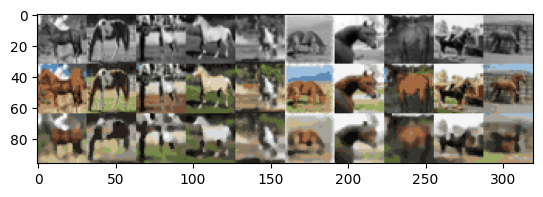
\includegraphics[scale=.75]{4.2.png}
\end{center}

\textbf{4.3:} Denoting $k$ as the kernel size, \begin{align*}
    \text{Total number of weights} &= k^2(NIC*NF + 2NF^2 + 2NF^2 + NF*NC + NC^2)\\
    &= k^2(NIC*NF + 4NF^2 + NF*NC + NC^2)\\
    \text{Total number of outputs} &= 32^2NF + 16^2NF + 16^2NF + 16^2(2NF) + 8^2(2NF) + 8^2(2NF)\\
    &+ 8^2NF + 16^2NF + 16^2NF + 16^2NC + 32^2NC + 32^2NC + 32^2NC\\
    &= 2880NF + 3328NC\\
    \text{Total number of connections} &= 32^2k^2NIC*NF + 32^2NF + 16^2NF + 16^2k^2*2NF^2 + 16^2*2NF\\
    &+ 8^2*2NF + 8^2k^2*2NF^2 + 16^2NF + 16^2NF + 16^2k^2NF*NC\\
    &+ 32^2NC + 32^2NC + 32^2k^2NC^2\\
    &= 1024k^2NIC*NF + 640k^2NF^2 + 256k^2NF*NC\\
    &+ 1024k^2NC^2 + 2432NF + 2048NC
\end{align*} If the input size is doubled, the total number of weights does not change, while the other two quantities increase by a factor of 4:\begin{align*}
    \text{Total number of weights} &= k^2(NIC*NF + 4NF^2 + NF*NC + NC^2)\\
    \text{Total number of outputs} &= 11520NF + 13312NC\\
    \text{Total number of connections} &= 4096k^2NIC*NF + 2560k^2NF^2 + 1024k^2NF*NC\\
    &+ 4096k^2NC^2 + 9728NF + 8192NC
\end{align*}

\textbf{5.1:} Refer to the notebook.

\textbf{5.2:} The resulting plot is shown below:
\begin{center}
    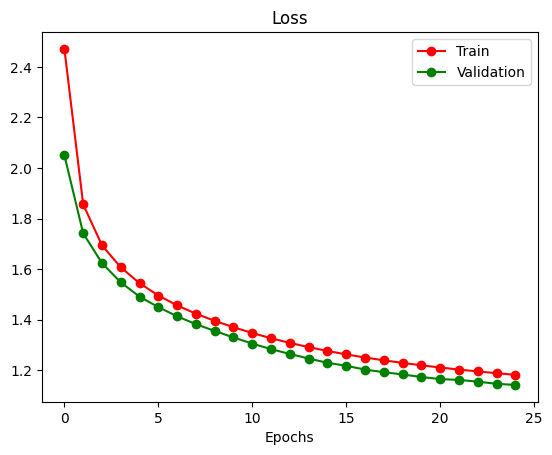
\includegraphics[scale=.75]{5.2.png}
\end{center}

\textbf{5.3:} The results are shown below; they look slightly better compared to before. At the end of training, the validation loss of the \texttt{ConvTransposeNet} model is lower than the loss of the \texttt{PoolUpsampleNet} model (1.1418 vs. 1.5791). This is likely because the max pool layers reduce the number of parameters and the upsampling layers do not increase them, while convolution transpose layers use more parameters and thus are able to learn more features.
\begin{center}
    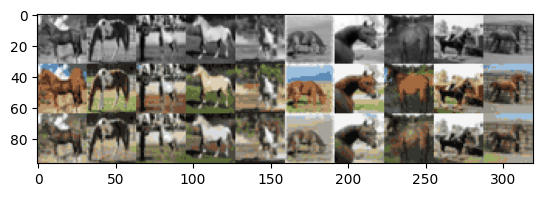
\includegraphics[scale=.75]{5.3.png}
\end{center}

\textbf{5.4:} For a kernel size of 4, \begin{itemize}
    \item the \texttt{padding} parameter for the \texttt{nn.Conv2d} layers should be 1;
    \item the \texttt{padding} parameter for the \texttt{nn.ConvTranpose2d} layers should be 1;
    \item and the \texttt{output\_padding} parameter for the \texttt{nn.ConvTranpose2d} layers should be 0.
\end{itemize} For a kernel size of 5, \begin{itemize}
    \item the \texttt{padding} parameter for the \texttt{nn.Conv2d} layers should be 2;
    \item the \texttt{padding} parameter for the \texttt{nn.ConvTranpose2d} layers should be 2;
    \item and the \texttt{output\_padding} parameter for the \texttt{nn.ConvTranpose2d} layers should be 1.
\end{itemize}

\end{document}